\documentclass[tikz,border=5mm]{standalone}
\usepackage{xcolor}

\begin{document}
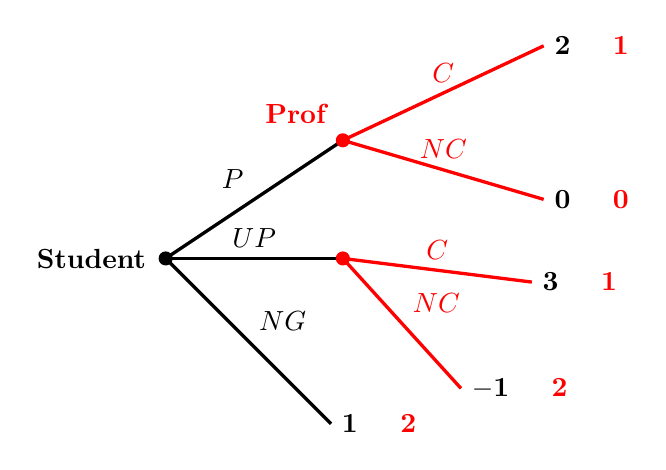
\begin{tikzpicture}[
    scale=1.5,
    font=\bfseries,
    dot/.style={circle, fill=#1, inner sep=1.8pt},
    dot/.default=black,
    line width=1.2pt
]

    % Coordinates
    \coordinate (root)   at (0, 0);
    \coordinate (qg_top) at (1.5, 1);
    \coordinate (qg_mid) at (1.5, 0);
    \coordinate (leaf_ng) at (1.4, -1.4);
    
    \coordinate (leaf1) at (3.2, 1.8);
    \coordinate (leaf2) at (3.2, 0.5);
    \coordinate (leaf3) at (3.1, -0.2);
    \coordinate (leaf4) at (2.5, -1.1);

    % Level 1 branches (You - Black)
    \draw[black] (root) -- (qg_top) node[midway, above left] {$P$};
    \draw[black] (root) -- (qg_mid) node[midway, above] {$UP$};
    \draw[black] (root) -- (leaf_ng) node[midway, above right] {$NG$};

    % Level 2 branches (QG - Red)
    \draw[red] (qg_top) -- (leaf1) node[midway, above] {$C$};
    \draw[red] (qg_top) -- (leaf2) node[midway, above] {$NC$};
    \draw[red] (qg_mid) -- (leaf3) node[midway, above] {$C$};
    \draw[red] (qg_mid) -- (leaf4) node[midway, above right] {$NC$};

    % Nodes & Labels
    \node[dot=black, label=left:Student] at (root) {};
    \node[dot=red, label={[red]above left:Prof}] at (qg_top) {};
    \node[dot=red] at (qg_mid) {};

    % Payoffs (You: black, QG: red)
    \node[right] at (leaf1) {2 \quad \textcolor{red}{1}};
    \node[right] at (leaf2) {0 \quad \textcolor{red}{0}};
    \node[right] at (leaf3) {3 \quad \textcolor{red}{1}};
    \node[right] at (leaf4) {$-$1 \quad \textcolor{red}{2}};
    \node[right] at (leaf_ng) {1 \quad \textcolor{red}{2}};

\end{tikzpicture}
\end{document}
